From a macroscopic perspective, nuclei can be viewed as charged particles, and thus collisions (here in a loose sense) between them is essentially governed by the Rutherford scattering formula.
This is how the nucleus was discovered in the first place. However, this simple picture breaks down at higher energies, when the de Broglie wave-length ($\lambda \sim \vec{p}^{-1}$) becomes sufficiently small to resolve the inner structure of the nuclei. At even higher energies, it becomes feasible to model the collision as not taking place between the two nuclei, but by individual protons and neutrons (nucleons).

This leads us to the \emph{participant-spectator} picture of nuclear collisions, in which the collision is viewed as if taking place between a few \emph{participant} nucleons, while the remaining \emph{spectator} nucleons remain mostly unaffected. Such a reaction is known as \emph{quasi-elastic scattering}, since the kinetic energy of the projectile will be much greater than the binding energy of the participants, which further motivates treating them as approximately free particles, and means that the kinetic energy will almost be conserved, hence \emph{quasi-elastic}.
!!!POSSIBLY DISCUSS LIMITATIONS!!!
The collision between the participant nucleons takes place at a time scale of about \unit[$10^{-23}$]{s}\cite{gaimard:1991:art}, and is sometimes called a \emph{fireball} or \emph{firestreak}.

However, this is just the first part of the collision. The participant nucleons may have gone unaffected through it, but the resulting system (a so-called pre-fragment) will be highly excited, and will decay to the actual fragment -- often by ejecting nucleons, in this context known as evaporating them. The characteristic time-scale for these ejections vary between \unit[$10^{-21}$ -- $10^{-16}$]{s}, depending on the energies and emitted particle\cite{gaimard:1991:art}. 

In this picture, we thus have a two-step process to describe nuclear fragmentation. 
Various models to describe both steps exist in the literature, which can be combined more or less freely---they do not necesarilly use the same paremeters to describe the nuclues. Models which mainly use parameters like $A$, the number of nucleons, $Z$ the number of protons, the total nuclear-spin $J$ and the excitation energy $E$ of the nucleus are termed \emph{macroscopic}, while models that directly treat the states of individual nucleons are called \emph{microscopic}. Examples of the former are the \emph{abrasion-ablation model}\cite{bowman:1973:book}, while the \emph{intranuclear-cascade model}\cite{metropolis:1991:art} is an example of a microscopic model. As is often the case in nuclear physics, no one model is valid of all range of nucleon number $A$ and incident energies\cite{cucinotta:1998:art}.

Since the focus on this report is to describe an event-generator for a physics experiment, we do not need a state of the art model (see !!!AUTOREF TO SECTION!!! for the arguments). Since the macroscopic properties of nuclei are more easily related to expermental observables, we will restrict our attention to those. 

\subsection{The fast processes -- the Goldhaber model}
!!! SUDDENLY, CODE. INTRODUCE MODEL FIRST? !!!
To mimic existing code !!!CITE LEONID?!!! and to allow the user to study a reaction of their interest, the outcome of the first stage of the process is largely determined by user input: the participant projectile nucleons -- the cluster -- as well as its invariant mass, and the excitation energy of the pre-fragment are both specified by user input. The only specific model used is to determine the momentum of the participant system relative to the projectile, everything else is just conservation of momentum, and an isotropic cross-section. 
The \emph{Goldhaber model} states that the momentum distribution is given by a Guassian with the width determined by the expectation value of the momentum of an individual nucleon, explicitly
\begin{equation}
\sigma^2 = \langle \vec{p}^2 \rangle A\frac{A_\text{p}-A}{A_\text{p}-1},
\end{equation}
where $A_\text{p}$ is the number of nucleons in the projectile, $A$ in the pre-fragment, and $\langle \vec{p}^2 \rangle$ is the expectation value of the momentum of an individual nucleon. For a Fermi-gas, $\langle \vec{p}^2 \rangle$ may be written in terms of the Fermi-momentum $\vec{p}_f$ as $\tfrac{3}{5} \vec{p}_f^2$\cite{goldhaber:1974:art}.
!!!THIS IS NOT THE MODEL USED IN LEONID CODE!!!


!!!LEONID USES
\begin{equation*}
\sigma^2 = 2 (M + m -M_p) \frac{mM}{m+M} = 2 Q \mu(m,M),
\end{equation*}
where $m$ is the mass of the participant, $M_p$ the mass of the projectile and $M$ the mass of the pre-fragment. If we take $Q=T = m v^2/2$, we get $\sigma^2 = m^2 v^2$, which could imply that this is just the Fermi-momentum?
!!!

!!!POSSIBLY MOVE NEXT TO CODE DOCUMENTATION, SINCE WHICH FRAME WE USE WHERE IS NOT REALLY GENERAL THEORY!!!
Momentum conservation implies that
\begin{align}
p_\text{p} &= p_\text{i} + q_\text{pf} \\
p_\text{i} + p_\text{t} &= q_\text{i} + q_\text{t}
\end{align}
where $p_\text{p}$ is the 4-momenum of the projectile, $p_\text{t}$ the momentum of the target, $p_\text{i}$ the internal momentum of the cluster; $q_\text{pf}$ the final momenum of the pre-fragment $q_\text{i}$ and $q_\text{t}$ the final momentum of the target and cluster, respectively.

Solving the above equation and squaring for $p_\text{i}$ and squaring gives an expression for the off-shell mass of the cluster as
\begin{equation}
p_\text{i}^2 = p_\text{p}^2 +  q_\text{pf}^2 -  p_\text{p}\cdot q_\text{pf}= m_\text{i}^2 =M_\text{p}^2 + M_\text{pf}^2 - M_\text{p}\sqrt{M_\text{pf} + \vec{p}_i^2},
\end{equation}
where we have evaluated $p_\text{p}\cdot q_\text{pf}$ in the rest-frame of the pre-fragment.

Since we are interested in constructing an event generator, we next transform the cluster's 4-momentum from the projectile to the laboratory frame (the projectile and target momentum is already known in the laboratory frame, the former being zero practically being a definition of that frame). The relevant gamma factor is
$\gamma = 1 + T/m_\text{p}$, where $T$ is the kinetic energy of the projectile.

Since the collision between the target and the cluster is easier to do in their zero-momentum (ZM) frame, we also need to transform between the laboratory and that frame. This is readily done by noting
\begin{equation}
\bar{\vec{P}} = \vec{p}_i + \vec{p}_t = \gamma(\beta_\text{ZM}) \bar{m} \beta_\text{ZM} = \bar{E}\beta_\text{ZM} \implies \beta_\text{ZM} = (\vec{p}_i + \vec{p}_t)/\bar{E},
\end{equation}
where $\bar{E}$ etc. denotes the energy of the system of both particles. Since we want the $\beta$ between the lab and the ZM frame, we evaluate all the quantities in the lab frame
\begin{equation}
\beta_\text{ZM} = \frac{\vec{p}_i}{E_\text{c} + m_\text{t}}. \label{eq:betazm}
\end{equation}

The scattering between target and cluster is back-to-back in the ZM frame, and we generate the scattering angle from an isotropic $\tfrac{d\sigma}{dt}$, which in practice means that the Mandelstam variable $t$ is a uniform random number. The ZM energy, momentum and scattering angle can be readily expressed in term of the invariant Mandelstam variables
\begin{align}
E_\text{c} &= \frac{s+m_\text{i} - m_\text{t}}{2\sqrt{s}} \\
|\vec{p}_\text{c}| &= \sqrt{E_\text{c}^2 - m_\text{i}^2} \\
\cos{\theta} &= \frac{t-m_\text{i}^2-m_\text{c}^2 + 2E_\text{c}^2}{2|\vec{p}_\text{c}|^2}.
\end{align}
A random polar angle $\phi$ in $[0,2\pi]$ is then generated, which together with $|\vec{p}_\text{c}|$, $\theta$ and $E_\text{c}$ fix the ZM 4-momentum of the cluster, and also the target by $\vec{p}_\text{t} = -\vec{p}_\text{c}$. Using \eqref{eq:betazm}, these results are boosted to the lab frame, in which we now have an expression for all the relevant momenta.

\subsection{The slow process -- decay of a compound nucleus}
There are at least two models for the decay of a compound nucleus popular in the literature, the Hauser-Feshbach and the Ewing-Weisskopf formulas. Both aim to describe how a compound nucleus in a given macro-state ($E*$, $J$, $Z$, $A$) will decay.

The older Ewing-Weisskopf formula, which this work is based on, gives the probability of decaying by evaporating a particle $\nu$ as
\begin{equation}
\frac{d^2 P_\nu}{dE_f dt} = \frac{1}{\hbar} \frac{\rho(E_f,J_f)}{\rho(E_i,J_i)} \sum_{S=|J_f-s|}^{|J_f+s|}\sum_{l=|J_i-S|}^{|J_i+S|} T_l(\epsilon_\nu),\qquad\cite{schmidt:1991:art}\label{eq:ew}
\end{equation}
where $P$ is the probability, $E_f$ the final-state energy, $J_f$ the final-state spin, $\rho$ the level densities and 
\begin{equation}
\epsilon_\nu \approx E_f-E_i-S_\nu\label{eq:kine}
\end{equation}
the kinetic energy of the evaporated particle, $S_\nu$ being its separation energy $S_\nu = M_f + m_\nu - M_i$\footnote{The approximation is due to neglecting the kinetic energy of the daughter nucleus, which should be a good approximation when the evaporated particle $\nu$ is light. This is not a necesary approximation, though, and a more exact formula is presented in !!!autoref!!!. The separation energy does not enter as a cost of removing the particle $\nu$, but rather to relate the two excitation energies $E_f$ and $E_i$ to an absolute scale.} . 
$s$ is the intrinsic spin of the evaporated particle, $S$ is the spin of the system consisting of the final state nucleus and evaporated particle, with $l$ being the orbital angular momentum of that state with respect to its center of mass. The sums give all the way to couple these while conserving the total angular momentum $\vec{J}_f+\vec{s} +\vec{l}= \vec{S} +\vec{l}= \vec{J}_i$. $T_l$ is the transition probability.
By integrating over $E$, we get $\frac{d P_\nu}{dt} = \Gamma_\nu$, which is roughly proportional to the probability to decay through the channel $\nu$, $P_\nu = \Gamma_\nu/\Gamma_{\text{tot}}$. 

Provided that the characteristic life-time of the system is short compared to the time resolution of the experimental setup, we may essentially treat the decay-widths as probabilities, since -- as far as the experiment is concerned -- the decay may as well take place instantenously. Note that the system may undergo multiple decays before it reaches its ground-state, and that time-scale of this entire decay chain must be short by the experimental standards. The time-of-flight resolution of the future \rtb{} setup will be in the picosecond range (\unit[$10^{-12}$]{s})\cite{r3b:online}, which is well above the time-scales of single evaporation given by Gaimard and Schmidt (\unit[$10^{-21}$ -- $10^{-16}$]{s})\cite{gaimard:1991:art}. Hence we will view $\Gamma_x$ as the probability to decay by a given process in an unspecified but short time step.

Since we are interested in simulating a decay chain, we want more information than merely the probability to decay by emitting a specific particle. We thus take a step back from \eqref{eq:ew}, and undo the summation over $l$
\begin{equation}
\frac{d\Gamma_{\nu,l}}{dE_f} = \frac{1}{\hbar} \frac{\rho(E_f,J_f)}{\rho(E_i,J_i)} \sum_{S=|J_f-s|}^{|J_f+s|} T_l(\epsilon_\nu),\label{eq:ew}
\end{equation}
which finally gives us the decay probability (per unit energy) from an initial state $(E_i,J_i)$ to a final state $(E_f,J_f)$ by emmiting a particle $\nu$ with angular momentum $l$ and momentum given by conservation of energy.

$\nu$ can in principle be any particles. However, the photon must be treated differently as it is massless and thus fully relativistic -- which makes the dististinction between $l$ and the intrinsic spin unnatural -- and removes a polarization state. With this in mind, we get
\begin{align}
&\frac{d\Gamma_{\gamma}}{dE_f} = \frac{1}{\hbar} \frac{\rho(E_f,J_f)}{\rho(E_i,J_i)} \sum_{l=|J_f-J_i|}^{|J_f+J_i|} T_l(\epsilon_\gamma) \\
\implies & \frac{d\Gamma_{\gamma,l}}{dE_f} = \frac{1}{\hbar} \frac{\rho(E_f,J_f)}{\rho(E_i,J_i)} T_l(\epsilon_\gamma),\label{eq:gammagamma}
\end{align}
where $l>0$ is an integer.

Although $\nu$ could be any particle, it becomes more appropriate to model the decay as a fission process if $\nu$ becomes sufficiently heavy in relation to the compound nucleus. Fission is usual modeled as a transition first to a \emph{transition state}, beyond which the nucleus will inevitably fission\cite{krane:book}. The present work does not include fission, and we will thus not discuss its details here. Swiateck discussed the possibility of treating particle emission and fission in an essentially symmetric fashion, by using a transition state formalism also for lighter particles\cite{swiatecki:1983:art}. !!MAY BE INTERESTING TO SAY SOMETHING ABOUT THIS. FIND SOURCE ON WHY THIS APPROACH ISN'T USED.!!

We will now describe models for the level density $\rho$ and transition probability $T_l$.

\subsubsection{Level densities}
The level density $\rho(E,J)$ enumerates the number of energy levels of a given nucleus in an energy range $[E,E+dE]$ with a given spin $J$. We have in our notation supressed the dependence on $A$ and $Z$. The nuclear level density increases rapidly with energy, which suggests that the nuclear levels are not simply built up by exciting single nucleons in a shell-model, since the spacing of these levels do not decrease nearly fast enough.

To see how the rapid increase in level densities may be accounted for by collective excitations, and to introduce some of the terminology, it is illustrative to have a look at a simple example.

\paragraph{The simple example}
Consider a ``nucleus'' in which we have $A$ identical nucleons, that occupy single particle states with spacing $d$. The situation is illustrated in \autoref{fig:equidist}. The energy of the nuclues is given by 
\begin{equation}
E=\sum_i \epsilon_i n_i,
\end{equation}
where $\epsilon = id$ is the energy of level $i$, and $n_i$ is the occupation number of that level, which can be $0$ or $1$, since nucleons are fermions.
If we take the Fermi energy as the reference energy, we get the excitation energy
\begin{equation}
E^*=\sum_i \epsilon_i n_i - \sum_i^A \epsilon_i n_i.
\end{equation}
The picture is more illustrative than the formulas. We now have one way to excite our system to $E^*=d$, namely by exciting the nucleon just below the Fermi level. For $E^*=2d$ we may proceed from our $E^*=d$ system in two ways, either by further exciting the lone excited nucleon $E^* = 2d$, or by exciting the highest nucleon in the $A-1$ system, $E^*=d+d$. For $E^*=3d$, we have
\begin{equation}
\begin{aligned}
1d+1d+1d \\
2d+1 \\
3d,
\end{aligned}
\end{equation}
and at this point, it should be apparent that we are really investigating the number of ways to write a natural number as a sum of natural numbers, a problem which engaged Euler as early as 1720\cite{mathworld}. It turns out to be a very rapidly growing function, with the number of ways to partition $100$ being $190 569 292$\cite{mathworld}.

!!!TODO: mention g=1/d and its relation to a.  Smearing out producedur by Laplace+saddle-point. Mention level vs density of states. !!!

\begin{figure}
\input{figures/rho-theory/equidistant.pdf_t}
\caption{\label{fig:equidist} Fermions with equidistant single-particle levels.}
\end{figure}

Since the level density increases very rapidly, it is reasonable to approximate it as a continuous function  for energies above the threshold for particle evaporation.
We use the following expression
\begin{equation}
\rho(E,J) = \frac{1}{\sqrt{2}24}
\frac{1}{\sigma a^{1/4} U^{5/4}} \exp{(2\sqrt{aU})}
\frac{2J+1}{\Theta_\text{eff}/(\hbar^2\beta)}\ exp{\left(-(J+\tfrac{1}{2})^2/(2\Theta_\text{eff}/(\hbar^2\beta))\right)},\label{eq:rho}
\end{equation}
which is a version of the widely-used expression for the level density of a \emph{Fermi gas} that takes angular momentum $J$ into account\cite{ripl:2006}.

Here, $U$ is an effective excitation energy above the \emph{yrast line}, corrected for shell and pairing effects. It is given by
\begin{equation}
U=E_\text{eff} + f(E_\text{eff})\delta S + g(E_\text{eff})\delta P,\label{eq:u}
\end{equation}
where $f$ and $g$ describes the damping of shell and pairing effects with increased energy, and $E_\text{eff} = E^*-E_\text{yrast}$. The \emph{yrast energy} is the lowest energy for a given angular momentum, here taken to be
\begin{equation}
E_\text{yrast} = \frac{(2J+1)\hbar^2}{2\Theta_\perp},
\end{equation}
corresponding to a quantum-mechanical axi-symmetric rotor rotating around its symmetry axis. This yrast energy is not strictly speaking the lowest energy for a given $J$, but the energy of a collective rotational excitation, which is a reasonable picture when we have many states with a given $J$ in our energy interval $[E,E+dE]$, which is needed for \eqref{eq:rho} to be valid. !!CITE. THIS IS A GUESS OF MINE. ALSO NOTE THAT THIS IS NOT AN ADDITIONAL ROTATIONAL DOF, SEE NUCLEAR STRUCTURE II BY BOHR + MOTTELSON.!!

The pairing energy $\delta P$ in \eqref{eq:u} can be estimated from the average separation energy for the surrounding nuclei (in an $(N,Z)$ plot, like an isotope chart), which is close to the actual observed shift between odd and even nuclei\cite{ericson:1960}. Neutrons and protons have different pairing energies, which is to be added or subtracted when neutron or proton number, respectively, is odd or even. 
The shell energy $\delta S$ can either be calculated from a microscopic model, or -- as I have done -- can be be estimated together with the pairing energy by comparing experimental masses with masses predicted by a macroscopic model, and taking the difference, as suggested by Schmidt and Morawek\cite{schmidt:1991:art}. I used the macroscopic part of the 1992 edition of the Finite-Range Droplet Model (FRDM-1992)\cite{moller1995}, which is presented in more detail in \autoref{sec:frdm1995}.

The damping of shell effects with energy can be described by an exponential function
\begin{equation}
f(E_\text{eff}) = 1-\exp{\left(-E_\text{eff}/E_\text{d}\right)},
\end{equation}
where $E_\text{d}$ is the shell-damping energy 
\begin{equation}
E_\text{d} = \frac{0.4}{a} A^{4/3},
\end{equation}
where $a$ is the level-density parameter, which for a spherical nuclei can be approximated by
\begin{equation}
a=\frac{A}{\unit[14.61]{MeV}}(1+3.114 A^{-1/3} + 5.626 A^{-2/3}).\qquad\cite{schmidt:1991:art}\label{eq:a}
\end{equation}
This parameter also enters directly into \eqref{eq:rho}.

Likewise, the damping of pairing effects with energy can also be described by a simple function, in this case
\begin{equation}
g(E_\text{eff}) = \begin{cases} 1-(1-E/E_\text{c})^2 & E_\text{eff} < E_\text{c} \\
 1 & E_\text{eff} \ge E_\text{c}.\qquad\cite{schmidt:1991:art}
\end{cases}
\end{equation}
The critical energy $E_\text{c}$ is approximately $\unit[10]{MeV}$ and varies with angular momentum, 
\begin{equation}
E_\text{c} = \unit[10]{MeV}\sqrt{1-(J/J_\text{c})^2},
\end{equation}
where the critical angular momentum $J_\text{c}$ is about $12\hbar$. !!!SOURCE FOR THIS?!!!

Since we have restricted ourselves to spherical nuclei in \eqref{eq:a}, we also have the moments of inertia $\Theta_\perp = \Theta_\parallel$. In particular, for a sphere with constant density, we have
\begin{equation}
\Theta = \frac{2}{5} M R_0^2 \approx \frac{2}{5} A^{5/3}\times u \times r_0^2
\end{equation}
The approximation is obtained by inserting $R_0 = r_0 A^{1/3}$ and $M=u A$, where $r_0=\unit[1.16]{fm}$ is the nuclear radius constant, with the same value as in the macroscopic model\cite{moller1995}. $u$ is the atomic mass units, $u \approx \unit[931.5]{MeV}$.

Finally, $\beta$ in \eqref{eq:rho} is the reciprocal nuclear temperature $\beta=1/T$\footnote{It really is the reciprocal temperature at the saddle-point, see e.g. Feldmeier\cite{grossjean1985}.}. It can be calculated from $\tfrac{a}{\beta}$, which is obtained by solving
\begin{equation}
a/\beta=\sqrt{(aU)[1 -exp{-a/\beta}]},\qquad\cite{grossjean1985}\label{eq:abiteration}
\end{equation}
which can be done numerically by iterating
\begin{equation}
(a/\beta)_{n+1}=\sqrt{aU[1 -exp{-(a/\beta)_n}]}
\end{equation}
from a suitable initial guess $(a/\beta)_{0}$. $(a/\beta)_{0}=\sqrt{aU}$ was used here, which solves \eqref{eq:abiteration} for $(a/\beta) \to \infty$ and is known to be a good initial guess\cite{grossjean1985}.

\def\bredd{0.5}

\begin{figure}
\begin{center}
\begin{tabular}{cc}
\subfloat[The level densities derived from \eqref{eq:rho}.]{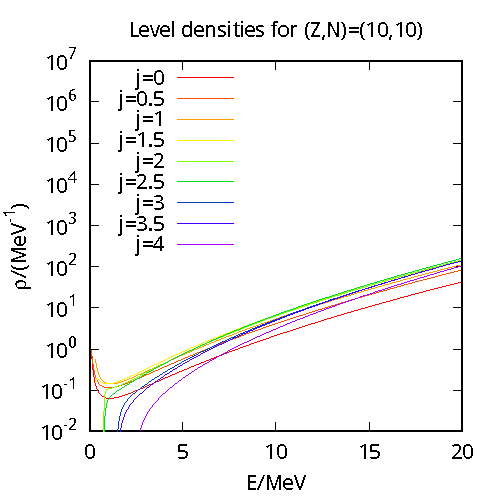
\includegraphics[width=\bredd\textwidth]{figures/rho/Z10N10.pdf}\label{sfig:rhoj:a}}
&
\subfloat[Without compensating for the yrast energy.]{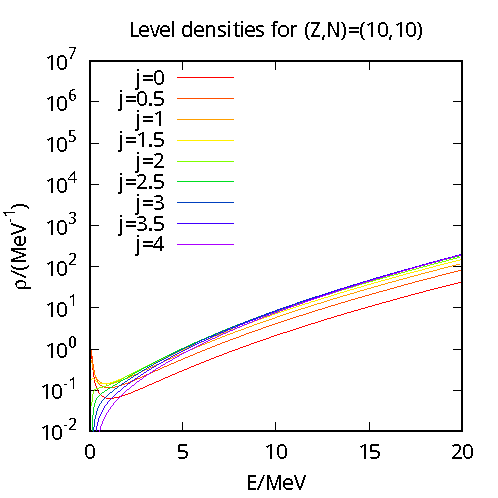
\includegraphics[width=\bredd\textwidth]{figures/rho/Z10N10_no-yrast.pdf}\label{sfig:rhoj:b}}
\end{tabular}
\caption{\label{fig:rhospin} The energy dependence of the level density of $~^{20}\mathrm{Ne}$ for spin $J=0,\tfrac{1}{2},\dots, 4$. In order to more easily be able to compare level densities for different spin at the same effective energy above the yrast line, the yrast energy has not been subtracted from $E_\text{eff}$ in \ref{sfig:rhoj:b}.}
\end{center}
\end{figure}


In order to get a picture of how all of this comes together, we have plotted the level density for the $A=10$ isobar for $J=0,\tfrac{1}{2},\dots, 4$. The level density of $~^{20}\mathrm{Ne}$ for different spin with and without subtracting the yrasy-energy is illustrated in \autoref{fig:rhospin}. 
As can be seen in the figure, the level densities for higher spin start at a lower value for low energies, way lower than $1$ level each $\unit{MeV}$ -- which indicates that the continous view of energy levels fails at these energies. 
The spins appear to be split up in $2$ groups, one for $J \le 1$ and one for $J>1$.
The level densities for $4 \ge J> 1$ initially grow rapidly, until they overtake the lower spin level densities and settle at a seemingly proportional relationship with each other. As a result of the $(2J+1)\exp{(J(J+1))}$ dependence on $J$, moderate $J$ values give the largest level density.
The same general behaviour is seen for the other nuclei at the $A=10$ isobar.

In order to see if this is a general feature of our model, we also investigate $~^{99}\mathrm{Zr}$ -- this nuclei being chosen arbitrarily as something far form the $A=10$ isobar. The corresponding plots of the level densities are seen in \autoref{fig:rhospin2}. We note that the inclusion of the yrast energy is not nearly as significant for the spins under consideration, since the larger value of $\Theta$ reduces the yrast energy of a given $J$. This also explains why $J=4$ has the highest density of states in this case: a higher $\Theta$ means that the $\exp{(J(J+1)/\Theta)}$ factor does not supress the level density as rapidly with increasing spin. 
We also see that it is only for $J\ge 3$ that we see the hint of a dip for lower energies. This could perhaps indicate that the pronounced spin-dependence seen for the $A=10$ isobar will reveal itself for yet higher spin -- a natural consequence of the higher moment of inertia for heavier nuclei.

\begin{figure}
\begin{center}
\begin{tabular}{cc}
\subfloat[The level densities derived from \eqref{eq:rho}.]{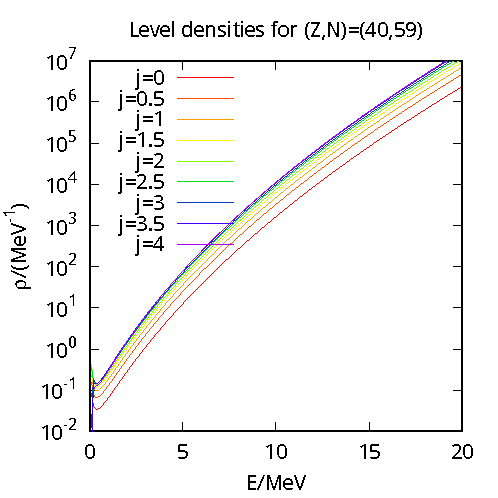
\includegraphics[width=\bredd\textwidth]{figures/rho/Z40N59.pdf}\label{sfig:rhoj2:a}}
&
\subfloat[Without compensating for the yrast energy.]{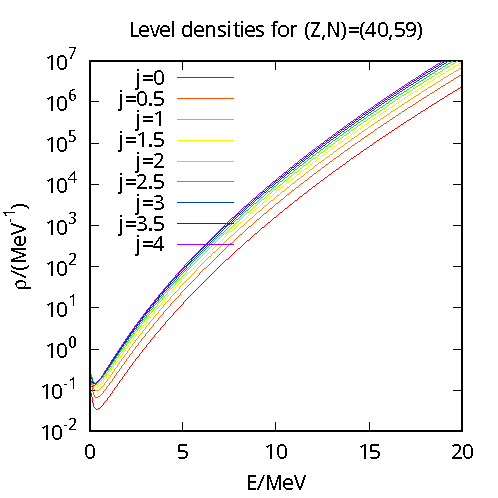
\includegraphics[width=\bredd\textwidth]{figures/rho/Z40N59_no-yrast.pdf}\label{sfig:rhoj2:b}}
\end{tabular}
\caption{\label{fig:rhospin2} The energy dependence of the level density of $~^{99}\mathrm{Zr}$ for spin $J=0,\tfrac{1}{2},\dots, 4$. In order to more easily be able to compare level densities for different spin at the same effective energy above the yrast line, the yrast energy has not been subtracted from $E_\text{eff}$ in \ref{sfig:rhoj2:b}.}
\end{center}
\end{figure}

In any case, this is low-energy behaviour, and both the Fermi gas model\cite{grossjean1985} and the very notion of a continuous level density has problems for low energies. Most notably, the Fermi gas model itself, without compensating for shell and pairing effects, predicts a singularity at $U=0$, which is why we see an increase in the level density for lower energies and spin in both \autoref{fig:rhospin2} and \autoref{fig:rhospin}, which have been truncated at $E=\unit[0.1]{MeV}$ in order to avoid this.

The level density was also investigated for a fixed spin for different nuclei on the $A=10$ isobar, but nothing conclusive was found.

On the other hand, for the isotope $Z=10$, the level density for higher energies generally increases with additional neutrons, which is to be expected, since there are more ways to arrange the nucleons for a give excitation energy, this is illustrated in \autoref{fig:Z10-rho}, where the brighter lines correspond to heavier nuclei.

\begin{figure}
\begin{center}
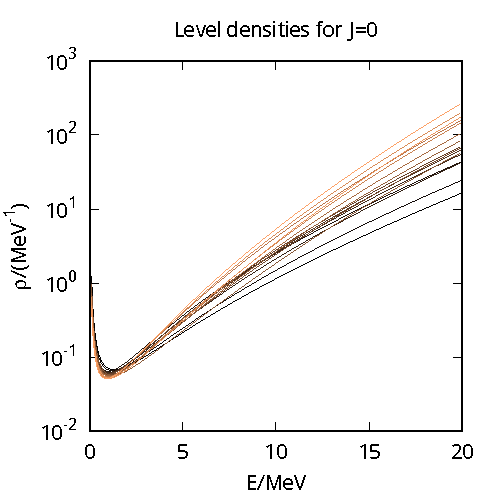
\includegraphics[width=\textwidth]{figures/rho/Z10_N7-N22.pdf}
\caption{\label{fig:Z10-rho} The level densities for $~^{17}\mathrm{Mg}$ to $~^{32}\mathrm{Mg}$, where brigther lines correspond to heavier nuclei.}
\end{center}
\end{figure}

\clearpage
\subsubsection{Transition Probabilities}
The decay width $\Gamma_{\nu,l}$ into a given final energy interval $[E_f,E_f+dE]$ by particle $\nu$ with orbital angular orbital momentum $l$ also depends on the transition probability $T_l(\epsilon_\nu)$.

One of the more well-known models of a transition probability by particle decay is the Gamow model for alpha decay, in which the mother nucleus $(Z,N)$ is modeled as essentially being composed of a ready-to-go alpha particle and the daughter nucleus $(Z-2,N-2)$ and the probability to decay is essentially given by the probability for the alpha particle to tunnel through the potential due to the daughter nucleus, with an additional factor depending on how often the alpha particle has a chance to tunnel. 

This model is readily generalized to other particle decays: we may just as well imagine a proton being formed inside the mother nucleus $(Z,N)$, and tunneling through the potential from the daughter nucleus $(Z-1,N)$.

In order to make this model quantitative, we need an actual potential. Approximating the charge distribution of the daughter and tunneling particle as spherical, we may model the potential due to electrostatic interaction as a simple Coulomb potential, which gives us
\begin{equation}
V = V_\text{Col} + \dots =  Z_1 Z_2 \frac{e^2}{r_{12}} + \dots,
\end{equation}
in non-rationalized units.
If we go ahead and assume that not only the charge distribution, but the potential as a whole is spherically symmetric, we can employ the standard procedure of splitting up the problem into a radial and angular part, where the radial potential is given by
\begin{equation}
V_\text{r} = Z_1 Z_2 \frac{e^2}{r_{12}} + \frac{l(l+1)\hbar^2}{2\mu r^2} + \dots
\end{equation}
where we still need additional terms to take into account the effective nucleon-nucleon intraction. The assumption of spherical symmetry also gives us the angular part of the wave function as a spherical harmonic, which gives us the angular distribution of the emitted particle in the center-of-mass frame.

\begin{figure}
\begin{center}
\input{figures/pot-theory/proximity.pdf_t}
\caption{\label{fig:prox} A schematic sketch of how the proximity approximation is carried out. Two close surfaces are approximated as a series of parallel surface, which in turn are approximated as infinite parallel surface, for which the potential energy is easier to calculate. This result is then summed up for all parallel surfaces.}
\end{center}
\end{figure}

The nuclear part of the potential used by \prgname{Codex} is a proximity potential\cite{gollerthan:1988:thesis}\cite{blocki1977}. 
Proximity potentials may be derived from a more general approximation method, in which two nearby surface are split up into parallel surface, close enough to be approximated as semi-infinite, see \autoref{fig:prox}\cite{fosco:2012}. The contributions from these different set of parallel surfaces are assumed to be additive.
The potential energy is calculated for these slabs, and factors to correct for the actual geometry are introduced. This approach is widely used in Casimir force calculations between objects of a more arbitrary shape\cite{fosco:2011}. This approximation is also known by ``Derjaguin approximation'' in other fields\cite{fosco:2012}.

In the nuclear case, the situation is somewhat complicated by the fact that the form of the nucleon-nucleon interaction is unknown. As such, there exist several proximity potentials\cite{dutt:2010}. Dutt et. al. showed that 12 common proximity potentials all were able to predict fusion barrier heights with $10\%$ of the experimental values for asymmetric fusion reactions ranging from $~^{12}\mathrm{C} + ~^{17}\mathrm{O}$ to $~^{86}\mathrm{Kr} + ~^{208}\mathrm{Pb}$\cite{dutt:2010}. Proximity-type potentials have also been used to explore alpha and proton decay\cite{proton-alpha-proxy:2005}\cite{proton-proxy:2010}, which is closer to our intended application\footnote{It is not immediately obvious to the author if the assumptions of the proximity potential formalism applies to proton or alpha decay. It does however reproduce experimental half-lives to a reasonable degree, see e.g. Balasubramaniam and Arunachala\cite{proton-alpha-proxy:2005} -- this is for emission from heavier nuclei, though.}.

The proximity potential is given by
\begin{equation}
V_\text{N} = C \phi(\zeta),\label{eq:vn}
\end{equation}
where $\phi(\zeta)$ is the so-called \emph{universal function}, which for a given nucleon-nucleon interaction is independent of the geometry of the nuclei in the proximity approximation. $\zeta$ is a unitless distance between the two nuclei, see below. Geometrical factors are contained in the proportionality ``constant'' $C$, which is given by
\begin{equation}
C = 4\pi \gamma b \frac{r_{c,1} r_{c,2}}{r_{c,1} + r_{c,2}}
\end{equation}
where $\gamma$ is the surface energy coefficient, which can be approximated by
\begin{equation}
\gamma= 0.9517 (1.0 - 1.78260 \times I^2),
\end{equation}
where $I=(N-Z)/A$ is the neutron excess.

We use the universal function due to Blocki 1997
\begin{equation}
\phi(\zeta)= \begin{cases}-0.5(\zeta-2.54)^2-0.0852(\zeta-2.54)^3 & \zeta < 1.2511 \\
-3.437\exp{(-\zeta/0.75)} & \zeta > 1.2511.\qquad\cite{blocki1977}
\end{cases}\label{eq:prox}
\end{equation}
$\zeta$ is the distance between the two nuclear surfaces, normalized with respect to the typical surface diffuseness of the nuclei, here taken to be $\unit[1]{fm}$\cite{blocki1977}. More explicitly, we have
\begin{equation}
\zeta = \frac{r - r_\text{sum}}{b},
\end{equation}
where $b$ is the surface diffuseness, and $r_\text{sum}$ is roughly the sum of the radii of the two nuclei, so that $r-r_\text{sum}$ gives the distance between the nuclear surfaces\cite{blocki1977}. An effective sharp nuclear surface may be estimated by the formula
\begin{equation}
r_\text{sharp} = 1.28 A^{1/3} - 0.76 + 0.8 A^{-1/3}\quad\units{fm}.\qquad\cite{blocki1977}\label{eq:sharp}
\end{equation}
%which in \prgname{CODEX} is adjusted by adding a radius correction constant, $r_\text{adj} = \unit[0.9]{fm}$.
\eqref{eq:sharp} is used to estimate the radii of all nuclei, and as a result $r_\text{sharp}=\unit[1.32]{fm}$ for protons and neutrons, which is slightly different from the value of $r_0$ that is normaly used.
%!!!  THE INPUT FILE SAYS ``VAZ ET. AL.'' NEXT TO RADIUS CORRECTION. WHAT IS THIS? !!!
In the proximity potential, it is preferable to use the \emph{central radius} $r_\text{c}$ rather than the effective sharp radius\cite{blocki1977}, which is given by 
\begin{equation}
r_\text{c} =r_\text{sharp} \left(1-\left(\trfac{b}{r_\text{sharp}}\right)^2\right)\quad.\qquad\cite{myers1973}
\end{equation}
Hence, $r_\text{sum} = r_\text{c,1}+r_\text{c,2}$. 

%!!!THIS WILL BE MORE CLEAR ONCE I WRITE SOMETHING GENERAL ABOUT THE MODEL, WHICH REALLY DEALS WITH BULK AND SURFACE ENERGIES OF A THIN-SKINNED SYSTEM.!!!

Since the proximity model takes the spartial extent of the nuclei into account, we modify the Coloumb-interaction accordingly, from that of a point particle to that of a homogenously charged ball
\begin{equation}
V_\text{C} = \begin{cases}\frac{Z_1 Z_2 e^2}{r} &\quad r>r_\text{ch} \\ \frac{Z_1 Z_2 e^2}{r_\text{ch}^2}(3-(r/r_\text{ch})^2) &\quad r<r_\text{ch}, \end{cases}
\end{equation}
where we here use the more common formula for the charge radius, $r_\text{ch} = r_0 A^{1/3}$.

 In \autoref{fig:np-Z10N10}, we illustrate the total potential from $~^{20}\mathrm{Ne}$ for tunneling of protons and neutrons. The individual contributions to the total potential may be discerned by looking at the potential for the emission of $l=0$ neutrons (which are only affected by the proximity potential) and $l=0$ protons (which have to tunnel through the sum of the Coulomb and proximity potential). %Since these potentials are only used for tunneling calculations, their shape below $E=0$ is not significant, since the particles cannot escape if their energy is less than $0$, and we will hence not display the $V<0$ parts in subsequent figures, in order to focus on the relevant details.
On this energy scale, the barrier protons have to tunnel through is merely \unit[2]{MeV} high, but since the proton separation energy for $~^{20}\mathrm{Ne}$ \unit[12]{MeV}, it will only happen for excitation above \unit[12]{MeV}, as the proton will not have a positive energy otherwise. Neutrons with a positive energy and $l=0$ will not have to tunnel at all, and instead will exist as resonances above the potential barrier. The tunneling formalism will not apply in this case, and we instead apply \eqref{eq:tlabove}, which we will touch upon later.

We also see that the centrifugal part quickly dominates, essentially a result of protons and neutrons being relatively light particles: for $\alpha$-decay, the centrifugal part is about a fourth of the values displayed above, and the $l$ dependence of the tunneling probability is not very significant\cite{weisskopf:1979}.  
This strong $l$ dependence makes proton radioactivity a sensitive probe to the orbital angular momentum of valence protons for proton emitting nuclei\cite{proton-alpha-proxy:2005}, but -- in this case -- it also poses a problem, since it removes the Coulomb+proximity barrier for high $l$-values. Even for moderate $l$ values, it makes particles with low energy classically forbidden inside the barrier, which appears inconsistent with the picture of a particle tunneling through a barrier.
The solution adopted in this work is to assign probability zero to tunnel for particles that are classically forbidden within the nucleus. This will supress decay for higher $l$, since the bottom of the potential well rises as $l$ does. For a higher $l$, the potential well disappears entirely\footnote{Another solution, attractive since we do not use the potential to estimate separation energies, is to model the strong interaction as an infinitely deep potential that cancels the centrifugal part, so that bound particles can always exist in the nucleus. The common $V=-\infty$ for $r<r_\text{nucleus}$ potential achieves this. Another solutions found in the literature is to have other, finite potentials below certain radii, but -- in non-relativistic quantum mechanics -- this goes against the assumption of spherical symmetry unless the effective nucleon-nucleon interaction depends on $l$ so to exactly cancel the centrifugal part.}.

\begin{figure}
\begin{center}
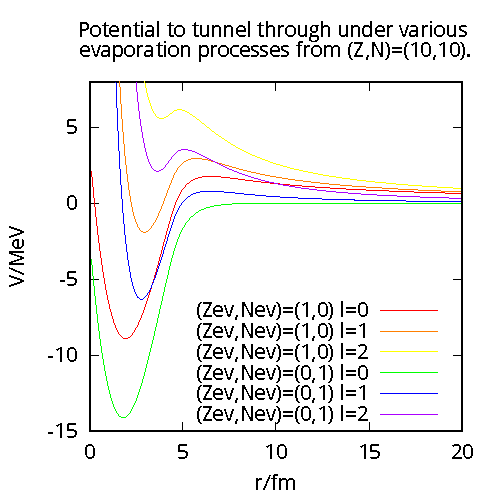
\includegraphics{figures/pot/np-potZ10N10.pdf}
\caption{\label{fig:np-Z10N10} The potential used for tunneling of neutrons and protons with $l=0,1,2$ from $~^{20}\mathrm{Ne}$. The potential for $l=0$ neutrons is exactly the proximity potential \eqref{eq:prox}, while the $l=0$ proton's potential show the sum of the proximity and Coulomb potential. }
\end{center}
\end{figure}

Given the potential, the transition probability can be calculated in the WKB approximation as 
\begin{equation}
T_l(\epsilon_\nu) = \exp{(-2G)},\qquad\cite{krane:book}
\end{equation}
where 
\begin{equation}
G=\sqrt{\frac{2\hbar}{\mu}} \int_{r_1}^{r_2} \sqrt{V_l(r)-\epsilon_{\nu}}\,dr.
\end{equation}
$r_1$ and $r_2$ are the inner and outer radii for which the kinetic energy is equal to the potential energy. It should be noted that the WKB approximation is not strictly speaking valid for regions where the potential is approximately constant over several wave-lengths $\lambda=\frac{2\pi}{k}$, which will not be valid for a classical turning point, since $\lambda \to \infty$. 
A somewhat more refined WKB approximation formula is
\begin{equation}
T_l(\epsilon_\nu) = \frac{1}{1+\exp{2G}},\qquad
\end{equation}
!!! CITE PAPER !!! which still suffers from the same short-comings as the previous formula. Nevertheless, the transition amplitudes calculated with the WKB formula are generally of the right order of magnitude, which should suffice for our purposes\cite{2011arXiv1106.1065N}.

For $\epsilon>V_\text{max}$, we can no longer view the emission as tunneling, as the particle passes ``over'' the barrier. Instead, we use
\begin{equation}
T_l = \frac{1}{1+\exp{\frac{2\pi}{\hbar \omega}(E-V_\text{max})}},\label{eq:tlabove}
\end{equation}
where
\begin{equation}
\hbar\omega = \hbar\sqrt{\frac{1}{\mu}\left(\frac{d^2V_l}{dr^2}\right)_{r_\text{max}}}.
\end{equation}
!!! MAYBE NEED TRANSLATION OF SECTION OF ULLI THESIS. CAN'T FIND SOURCE !!!

\paragraph{\gamma-decay}
The above discription concerned the tunneling of a nucleon or cluster through a potential barrier, and is thus not applicable to gamma decay.

$\gamma$-ray strength functions $f_{XL}$ can be used to calculate transition probabilities by $\gamma$-ray emission, 
\begin{equation}
T_L(E) = E^{2L+1} f_{XL}(E),\label{eq:gammat}
\end{equation}
where $f_l$ in principle can depend on whether the transition is electric or magnetic, $X=E$ and $X=M$, respectively. Viewed experimentally, \eqref{eq:gammat} can almost be viewed as a definition of the strength function. For exemple, the definition in the \emph{Gamma-Ray Strength Functions} in the book \emph{Advances in Nuclear Physics}\cite{ainp:1973}, defines the strength function as
\begin{equation}
f_{ifXL}^J = \frac{\bar{\Gamma_{ifXL}}}{E^{2L+1}_\gamma}\rho_{J}(E_i),
\end{equation}
and if we take $f_{XL}$ to be independent of $J$ and recall the definition of $\Gamma$ \eqref{eq:gammagamma}, we find that the definitions agree up to a factor $\rho_J(E_f)/\hbar$, which is essentially a constant for a fixed final state, as considered above.

The transmission coefficient used by \prgname{CODEX} ... !!!TODO!!!
